\documentclass[aspectratio=169,11pt]{beamer}

\usepackage{graphicx}
\usepackage{tikz}
\usetikzlibrary{positioning,arrows.meta}
\usepackage{xcolor}
\usepackage{booktabs}
\usepackage{tabularx}
\usepackage{array}
\usepackage{ragged2e}

\definecolor{GEUBlue}{RGB}{20,55,105}
\definecolor{GEULightBlue}{RGB}{238,244,251}
\definecolor{GEUGrey}{RGB}{90,90,90}
\definecolor{GEULightGrey}{RGB}{245,246,248}

\usetheme{default}
\setbeamertemplate{navigation symbols}{}
\setbeamertemplate{blocks}[rounded][shadow=false]
\setbeamercolor{normal text}{fg=black,bg=white}
\setbeamercolor{frametitle}{fg=GEUBlue}
\setbeamercolor{structure}{fg=GEUBlue}
\setbeamercolor{block title}{fg=GEUBlue,bg=GEULightBlue}
\setbeamercolor{block body}{fg=black,bg=GEULightBlue}
\setbeamerfont{frametitle}{size=\Large,series=\bfseries}

% Replace with the actual logo filename
\newcommand{\GEULogo}{graphicera_logo.png}

% Header and footer
\setbeamertemplate{headline}{%
  \begin{tikzpicture}[remember picture,overlay]
    \node[anchor=north east,xshift=-0.30cm,yshift=-0.12cm]
      at (current page.north east)
      {\includegraphics[height=0.62cm]{\GEULogo}};
  \end{tikzpicture}
  \vspace{0.72cm}
}
\setbeamertemplate{frametitle}{%
  \vspace{0.03cm}
  \insertframetitle\par
  \vspace{0.04cm}
  \textcolor{GEUBlue}{\rule{\textwidth}{0.9pt}}
  \vspace{0.03cm}
}
\setbeamertemplate{footline}{%
  \leavevmode
  \hbox{%
  \begin{beamercolorbox}[wd=.82\paperwidth,ht=0.32cm,dp=0.10cm,leftskip=.3cm]{author in head/foot}
    \tiny Department of Computer Science \& Engineering | Graphic Era (Deemed to be University)
  \end{beamercolorbox}%
  \begin{beamercolorbox}[wd=.18\paperwidth,ht=0.32cm,dp=0.10cm,rightskip=.3cm]{date in head/foot}
    \hfill\tiny\insertframenumber/\inserttotalframenumber
  \end{beamercolorbox}}
}

\newcommand{\smallnote}[1]{\vspace{0.08cm}{\scriptsize\color{GEUGrey}#1}}
\newcommand{\placeholder}[1]{\textit{\color{GEUGrey}#1}}

\title{\textbf{Project-Based Learning}\\[2mm]\large Phase-I Evaluation}
\author{\textbf{Project Title}\\Team ID: XXXX}
\institute{Department of Computer Science \& Engineering\\Graphic Era (Deemed to be University), Dehradun}
\date{Academic Session 2026--27}

\begin{document}

% 1
\begin{frame}[plain]
\begin{tikzpicture}[remember picture,overlay]
\draw[GEUBlue,line width=3pt] (current page.north west) -- (current page.north east);
\node[anchor=north east,xshift=-0.45cm,yshift=-0.35cm] at (current page.north east)
{\includegraphics[height=1.0cm]{\GEULogo}};
\node[align=center,text width=.84\paperwidth] at ([yshift=.25cm]current page.center)
{{\color{GEUBlue}\fontsize{26}{30}\selectfont\bfseries PROJECT-BASED LEARNING}\\[3mm]
 {\fontsize{18}{22}\selectfont PHASE-I EVALUATION}\\[7mm]
 {\color{GEUGrey}\Large\bfseries \placeholder{Project Title}}\\[3mm]
 {\color{GEUBlue}\normalsize Team ID: XXXX}};
\node[align=center,anchor=south,yshift=.42cm] at (current page.south)
{\bfseries Department of Computer Science \& Engineering\\
Graphic Era (Deemed to be University), Dehradun\\[-1mm]
\scriptsize Academic Session 2026--27};
\end{tikzpicture}
\end{frame}

% 2
\begin{frame}{Team \& Mentor Details}
\begin{columns}[T,totalwidth=\textwidth]
\column{.48\textwidth}
\begin{block}{Team Information}
\begin{tabular}{@{}ll@{}}
\textbf{Team ID:} & XXXX\\
\textbf{Semester:} & 3rd / 5th\\
\textbf{Section:} & XX\\
\textbf{Domain:} & \placeholder{XXXX}
\end{tabular}
\end{block}
\column{.48\textwidth}
\begin{block}{Team Members}
1.\quad \placeholder{Siddhant -- ID}\\
2.\quad \placeholder{Student Name -- ID}\\
3.\quad \placeholder{Student Name -- ID}\\
4.\quad \placeholder{Student Name -- ID}
\end{block}
\end{columns}
\vspace{2mm}
\begin{block}{Mentor}
\placeholder{Dr. / Mr. / Ms. Mentor Name}
\hfill
\textbf{Interactions completed:} \underline{\hspace{12mm}}
\end{block}
\end{frame}

% 3
\begin{frame}{Problem Statement \& Motivation}
\begin{block}{Problem Statement}
\placeholder{Clearly describe the real-world problem, its context, and the specific gap that the project intends to address.}
\end{block}
\vspace{2mm}
\begin{columns}[T,totalwidth=\textwidth]
\column{.48\textwidth}
\textbf{\color{GEUBlue}Motivation}
\begin{itemize}\itemsep2pt
\item \placeholder{Current limitation / gap}
\item \placeholder{Impact on users or organizations}
\item \placeholder{Limitations of existing approaches}
\end{itemize}
\column{.48\textwidth}
\textbf{\color{GEUBlue}Target Users / Stakeholders}
\begin{itemize}\itemsep2pt
\item \placeholder{Primary users}
\item \placeholder{Secondary stakeholders}
\item \placeholder{Expected benefit}
\end{itemize}
\end{columns}
\end{frame}

% 4
\begin{frame}{Objectives}
\textbf{\color{GEUBlue}Project Objectives}
\vspace{2mm}
\begin{enumerate}\itemsep5pt
\item \placeholder{Develop a solution for the identified problem.}
\item \placeholder{Implement the proposed core functionality.}
\item \placeholder{Integrate concepts from both PBL subjects.}
\item \placeholder{Evaluate the system using suitable metrics or test cases.}
\item \placeholder{Demonstrate practical applicability and future scope.}
\end{enumerate}
\vfill
\begin{center}
\colorbox{GEULightBlue}{\parbox{.80\textwidth}{\centering
\textbf{Key Objective:} \placeholder{State the main measurable outcome of the project.}}}
\end{center}
\end{frame}

% 5
\begin{frame}{Proposed Solution}
\begin{columns}[T,totalwidth=\textwidth]
\column{.48\textwidth}
\textbf{\color{GEUBlue}Proposed Approach}
\begin{enumerate}\itemsep3pt
\item \placeholder{Input / Data Collection}
\item \placeholder{Processing / Core Algorithm}
\item \placeholder{System Logic}
\item \placeholder{Database / Storage}
\item \placeholder{Output / Visualization}
\end{enumerate}
\column{.48\textwidth}
\textbf{\color{GEUBlue}Key Features}
\begin{itemize}\itemsep3pt
\item \placeholder{Feature 1}
\item \placeholder{Feature 2}
\item \placeholder{Feature 3}
\item \placeholder{Feature 4}
\item \placeholder{Feature 5}
\end{itemize}
\end{columns}
\vfill
\smallnote{Clearly explain how the proposed solution addresses the identified problem.}
\end{frame}

% 6
\begin{frame}{Integration of PBL Course Concepts}
\scriptsize
\begin{center}
\renewcommand{\arraystretch}{1.25}
\begin{tabularx}{.96\textwidth}{@{}>{\bfseries}p{3.0cm}X p{2.5cm}@{}}
\toprule
Course & Concepts Applied & Project Module\\
\midrule
Data Structures in C & \placeholder{Arrays, Linked Lists, Trees, Graphs, Hashing, etc.} & \placeholder{Module X}\\
OOPs with C++ & \placeholder{Classes, Inheritance, Polymorphism, STL, etc.} & \placeholder{Module Y}\\
\midrule
Operating Systems & \placeholder{Processes, Scheduling, Memory, Synchronization, etc.} & \placeholder{Module X}\\
DBMS & \placeholder{SQL, Transactions, Normalization, Indexing, etc.} & \placeholder{Module Y}\\
\bottomrule
\end{tabularx}
\end{center}
\vfill
\begin{center}
\colorbox{GEULightBlue}{\parbox{.86\textwidth}{\centering
\textbf{Requirement:} Demonstrate meaningful integration of both subjects in \textbf{one} project.}}
\end{center}
\end{frame}

% 7
\begin{frame}{System Architecture / Workflow}
\begin{center}
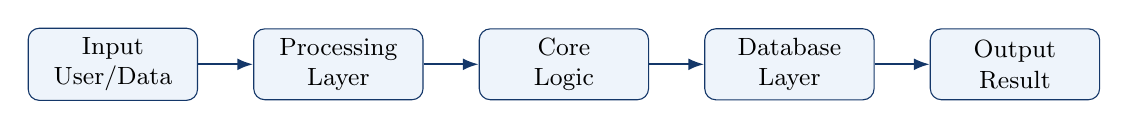
\begin{tikzpicture}[
node distance=7mm,
box/.style={rectangle,rounded corners,draw=GEUBlue,fill=GEULightBlue,
minimum width=2.15cm,minimum height=9mm,align=center,font=\small},
arrow/.style={-{Latex[length=2mm]},thick,draw=GEUBlue}
]
\node[box] (a) {Input\\User/Data};
\node[box,right=of a] (b) {Processing\\Layer};
\node[box,right=of b] (c) {Core\\Logic};
\node[box,right=of c] (d) {Database\\Layer};
\node[box,right=of d] (e) {Output\\Result};
\draw[arrow] (a)--(b); \draw[arrow] (b)--(c); \draw[arrow] (c)--(d); \draw[arrow] (d)--(e);
\end{tikzpicture}
\end{center}
\vspace{5mm}
\begin{columns}[T,totalwidth=\textwidth]
\column{.48\textwidth}
\textbf{\color{GEUBlue}Major Components}
\begin{itemize}\itemsep2pt
\item \placeholder{Component / Module 1}
\item \placeholder{Component / Module 2}
\item \placeholder{Component / Module 3}
\end{itemize}
\column{.48\textwidth}
\textbf{\color{GEUBlue}Data / Control Flow}
\begin{itemize}\itemsep2pt
\item \placeholder{How data moves through the system}
\item \placeholder{How modules interact}
\item \placeholder{Expected output}
\end{itemize}
\end{columns}
\end{frame}

% 8
\begin{frame}{Technology Stack \& Methodology}
\begin{columns}[T,totalwidth=\textwidth]
\column{.48\textwidth}
\begin{block}{Technology Stack}
\begin{itemize}\itemsep2pt
\item Programming: \placeholder{C / C++ / Other}
\item Database: \placeholder{MySQL / PostgreSQL}
\item Tools / Framework: \placeholder{XXXX}
\item IDE: \placeholder{XXXX}
\item Version Control: \placeholder{Git / GitHub}
\end{itemize}
\end{block}
\column{.48\textwidth}
\begin{block}{Development Methodology}
\begin{enumerate}\itemsep2pt
\item Requirement Analysis
\item System Design
\item Implementation
\item Testing
\item Evaluation
\end{enumerate}
\end{block}
\end{columns}
\vfill
\begin{center}
\smallnote{Justify the selection of technologies and methodology.}
\end{center}
\end{frame}

% 9
\begin{frame}{Initial Progress \& Team Contribution}
\begin{columns}[T,totalwidth=\textwidth]
\column{.44\textwidth}
\textbf{\color{GEUBlue}Progress Achieved}
\begin{itemize}\itemsep3pt
\item \placeholder{Background / literature study}
\item \placeholder{Requirements identified}
\item \placeholder{Architecture prepared}
\item \placeholder{Initial module implemented}
\item \placeholder{Database / data preparation}
\end{itemize}
\column{.52\textwidth}
\textbf{\color{GEUBlue}Individual Contribution}
\vspace{2mm}
\scriptsize
\begin{tabularx}{\textwidth}{@{}p{1.8cm}p{2.0cm}X@{}}
\toprule
Member & Role & Contribution\\
\midrule
\placeholder{M1} & \placeholder{Lead} & \placeholder{XXXX}\\
\placeholder{M2} & \placeholder{Developer} & \placeholder{XXXX}\\
\placeholder{M3} & \placeholder{DB/Testing} & \placeholder{XXXX}\\
\placeholder{M4} & \placeholder{Developer/Docs} & \placeholder{XXXX}\\
\bottomrule
\end{tabularx}
\end{columns}
\end{frame}

% 10
\begin{frame}{Roadmap, Expected Outcomes \& References}
\begin{columns}[T,totalwidth=\textwidth]
\column{.47\textwidth}
\textbf{\color{GEUBlue}Roadmap}
\begin{enumerate}\itemsep3pt
\item Phase-I: Proposal \& Design
\item Phase-II: Development
\item Phase-III: Final Implementation
\end{enumerate}
\vspace{2mm}
\textbf{\color{GEUBlue}Expected Outcomes}
\begin{itemize}\itemsep2pt
\item \placeholder{Working prototype / system}
\item \placeholder{Measurable results}
\item \placeholder{Practical applicability}
\item \placeholder{Future scalability}
\end{itemize}
\column{.47\textwidth}
\textbf{\color{GEUBlue}References}
\begin{enumerate}\itemsep3pt
\item \placeholder{Research paper / journal}
\item \placeholder{Book / standard}
\item \placeholder{Official documentation}
\item \placeholder{Dataset / repository}
\end{enumerate}
\vfill
\begin{center}
\colorbox{GEUBlue}{\parbox{.78\textwidth}{\centering\color{white}\textbf{Thank You}\\Questions \& Suggestions}}
\end{center}
\end{columns}
\end{frame}

\end{document}
